\subsection{RGB-D 相机}

% \subsubsection{简介}
\par RGB-D(Red Green Blue-Depth)相机是一种深度感知设备,它能够捕捉RGB图像以及与之对应的深度信息,主要有结构光(Structured
Light)\cite{structuredlight}和飞行时间(Time Of Flight, ToF)\cite{timeoflight}两种工作原理。
截至目前,RGB-D相机在许多领域都得到了广泛的应用:

\paragraph{三维重建}
\par RGB-D相机为三维重建提供了详细的场景信息,包括物体的形状、纹理和距离。这使得RGB-D相机在实时建模、室内建筑物扫描以及增强现实(Augmented
Reality, AR)和虚拟现实(Virtual Reality, VR)等领域具有广泛应用\cite{kim2016real,endres20133}。

\paragraph{机器人导航和定位}
\par 利用RGB-D相机获取的深度信息,机器人可以在复杂环境中进行精确的定位和自主导航。这对于服务机器人、工业机器人以及无人驾驶等应用领域具有重要意义\cite{taketomi2017visual,EfficientRGB-DSLAM}。

\paragraph{手势识别和人体姿态估计}
\par RGB-D相机为人体姿态估计和手势识别提供了三维数据,可以帮助计算机更准确地识别人体动作。这在游戏、医疗诊断和虚拟现实等领域具有广泛应用\cite{kim2016real,supancic2015depth,ge2018real}。

% \paragraph{人机交互}
% \par RGB-D相机为人机交互提供了更丰富的信息,使得交互方式更加多样化和自然。这对于虚拟现实、增强现实、智能家居等领域具有重要价值。

% \begin{figure}[htb]
% 	\centering
% 	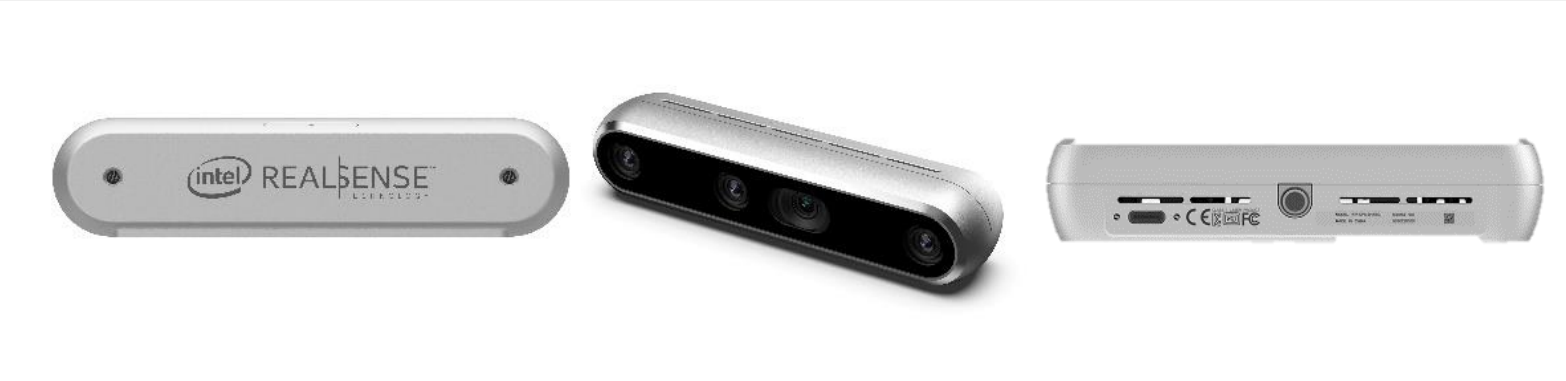
\includegraphics[width=0.9\textwidth]{figures/d455_example.png}
% 	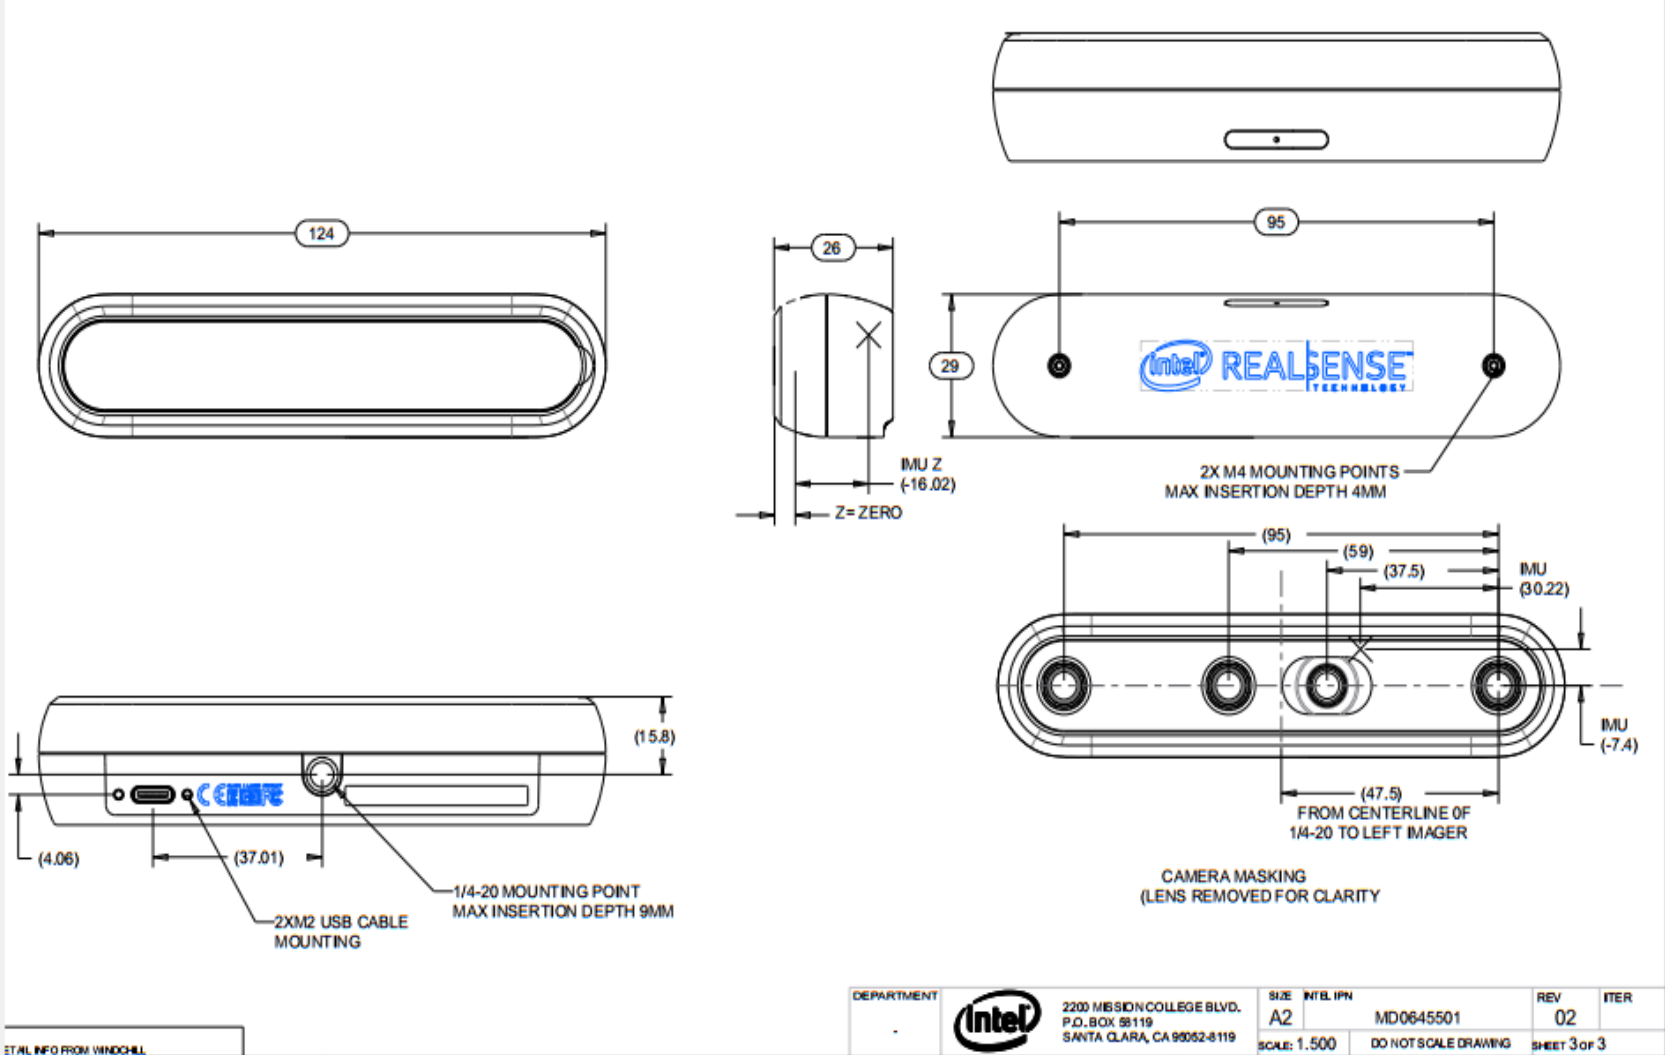
\includegraphics[width=0.9\textwidth]{figures/d455_structure.png}
% 	\caption{Intel ReadSense Depth Camera D455相机结构}
% 	\note{注:Intel RealSense Depth Camera D455 深度相机集成了一对立体深度传感器,一个RGB摄像头,以及一个内建的IMU惯性测量单元,摄像头的前面板标注有各种传感器和组件的名称和位置。该相机的每一个元素都设计得精巧紧凑,以提供高精度的深度感知能力,适应多种应用场景。}
% 	\label{fig:d455_example}
% \end{figure}
% \subsubsection{Intel ReadSense相机}

\par 在众多RGB-D相机品牌中,Intel RealSense 是一款备受欢迎的选择。Intel RealSense 由英特尔公司开发,具备实时3D扫描和物体识别功能,使设备能够与现实世界进行更自然、更直观的交互。
这款相机采用红外线投影仪和深度传感器捕捉物体的深度信息,实现场景的3D扫描和物体识别。同时,它能够捕捉高分辨率的RGB图像和深度图像,为用户提供丰富的视觉数据。
Intel
RealSense具有较高的计算性能,能够实时处理大量深度数据,为应用程序提供即时反馈。为了方便开发者快速集成RealSense技术,英特尔公司为其提供了一套全面的软件开发工具包(Software
Development Kit,SDK), 包括多种编程语言的应用程序接口(Application Program
Interface,API)、示例代码和文档等。此外,Intel
RealSense具有模块化设计,可根据不同的应用需求选择合适的模组进行组合,同时支持多种操作系统(如Windows、Linux、Android等),与各种硬件平台无缝集成。
目前,该型机的最新型号为Intel ReadSense Depth Camera
D455,技术规格见表~\ref{Intel_ReadSense_Depth_Camera_D455}。

\begin{table}[htb]
	\centering
	\caption{\href{https://www.intelrealsense.com/zh-hans/depth-camera-d455/}{Intel ReadSense Depth Camera D455 技术规格}}
	\label{Intel_ReadSense_Depth_Camera_D455}
	\begin{tabular}{c|ll}
		\toprule
		类型                   & \multicolumn{2}{c}{属性}                                                                                                                                    \\

		\midrule
		\multirow{2}{*}{特性}  & 使用环境:室内 / 室外                                                                        & 推荐范围:0.6 $\textasciitilde$ 6 m                                      \\
		                     & 深度快门类型:全局快门                                                                         & 惯性量测单元:Bosch BMI055                                                 \\

		\midrule
		\multirow{3}{*}{深度}  & 深度技术:立体                                                                             & 深度视场(FOV):\SI{87}{\degree} $\times$ \SI{58}{\degree}                \\
		                     & 最小深度距离 (Min-Z):$\textasciitilde$ 0.52 m                                             & 深度输出分辨率:高达 1280 $\times$ 720                                        \\
		                     & 深度精度< 2\%位于4 m                                                                      & 深度帧率:高达90帧/秒                                                        \\

		\midrule
		\multirow{3}{*}{RGB} & RGB帧分辨率:高达 1280 $\times$ 800                                                        & RGB 传感器 FOV (H \times V):\SI{90}{\degree} $\times$ \SI{65}{\degree} \\
		                     & RGB 帧速率:30 帧/秒                                                                      & RGB传感器分辨率:1 MP                                                      \\
		                     & RGB 传感器技术:全局快门                                                                      &                                                                     \\

		\midrule
		主要组件                 & 摄像头模块:英特尔实感模块 D450                                                                  & 计算处理器板:英特尔实感视觉处理器 D4                                                \\

		\midrule
		\multirow{3}{*}{物理}  & 外形:摄像头外设                                                                            & 接头:USB‑C* 3.1 Gen 1*                                                \\
		                     & \multicolumn{2}{l}{长度 $\times$ 深度 $\times$ 高度:124 mm $\times$ 26 mm $\times$ 29 mm}                                                                       \\
		                     & \multicolumn{2}{l}{安装机构:一个 1/4‑20 UNC 螺纹安装点、两个 M3 螺纹安装点、三脚架}                                                                                              \\

		\bottomrule
	\end{tabular}
	\note{注:深度精度是出厂测量值}
\end{table}

\par 在未来,RGB-D相机将会有很多可能的发展和改进方向。
为了满足更高精度和分辨率的需求,RGB-D 相机的硬件和算法将继续发展,未来会提供更高的深度精度,更细致的深度分辨率以及更低的噪声。
随着技术的进步,RGB-D相机将变得更小、更轻便,甚至被被集成到智能手机、平板电脑和其他便携式设备中\cite{alkhawaja_jaradat_romdhane_2023},这将进一步推动增强现实和虚拟现实的发展。
另一方面,为了在各种光照条件下保持良好的性能,RGB-D相机将会继续改进以克服环境干扰\cite{EfficientRGB-DSLAM},包括开发新的光学镜头、改进传感器技术以及设计更强大的算法以处理复杂环境中的数据。

\par 随着RGB-D相机技术的不断发展,它们将在新的应用领域得到广泛应用\cite{rgbd_ad,rgbd_respiratory}。
在未来,RGB-D相机的影响将不仅仅局限于影像采集和处理,更可能会改变我们与世界的交互方式。